\begin{figure}[H]
\centering
\subfigure{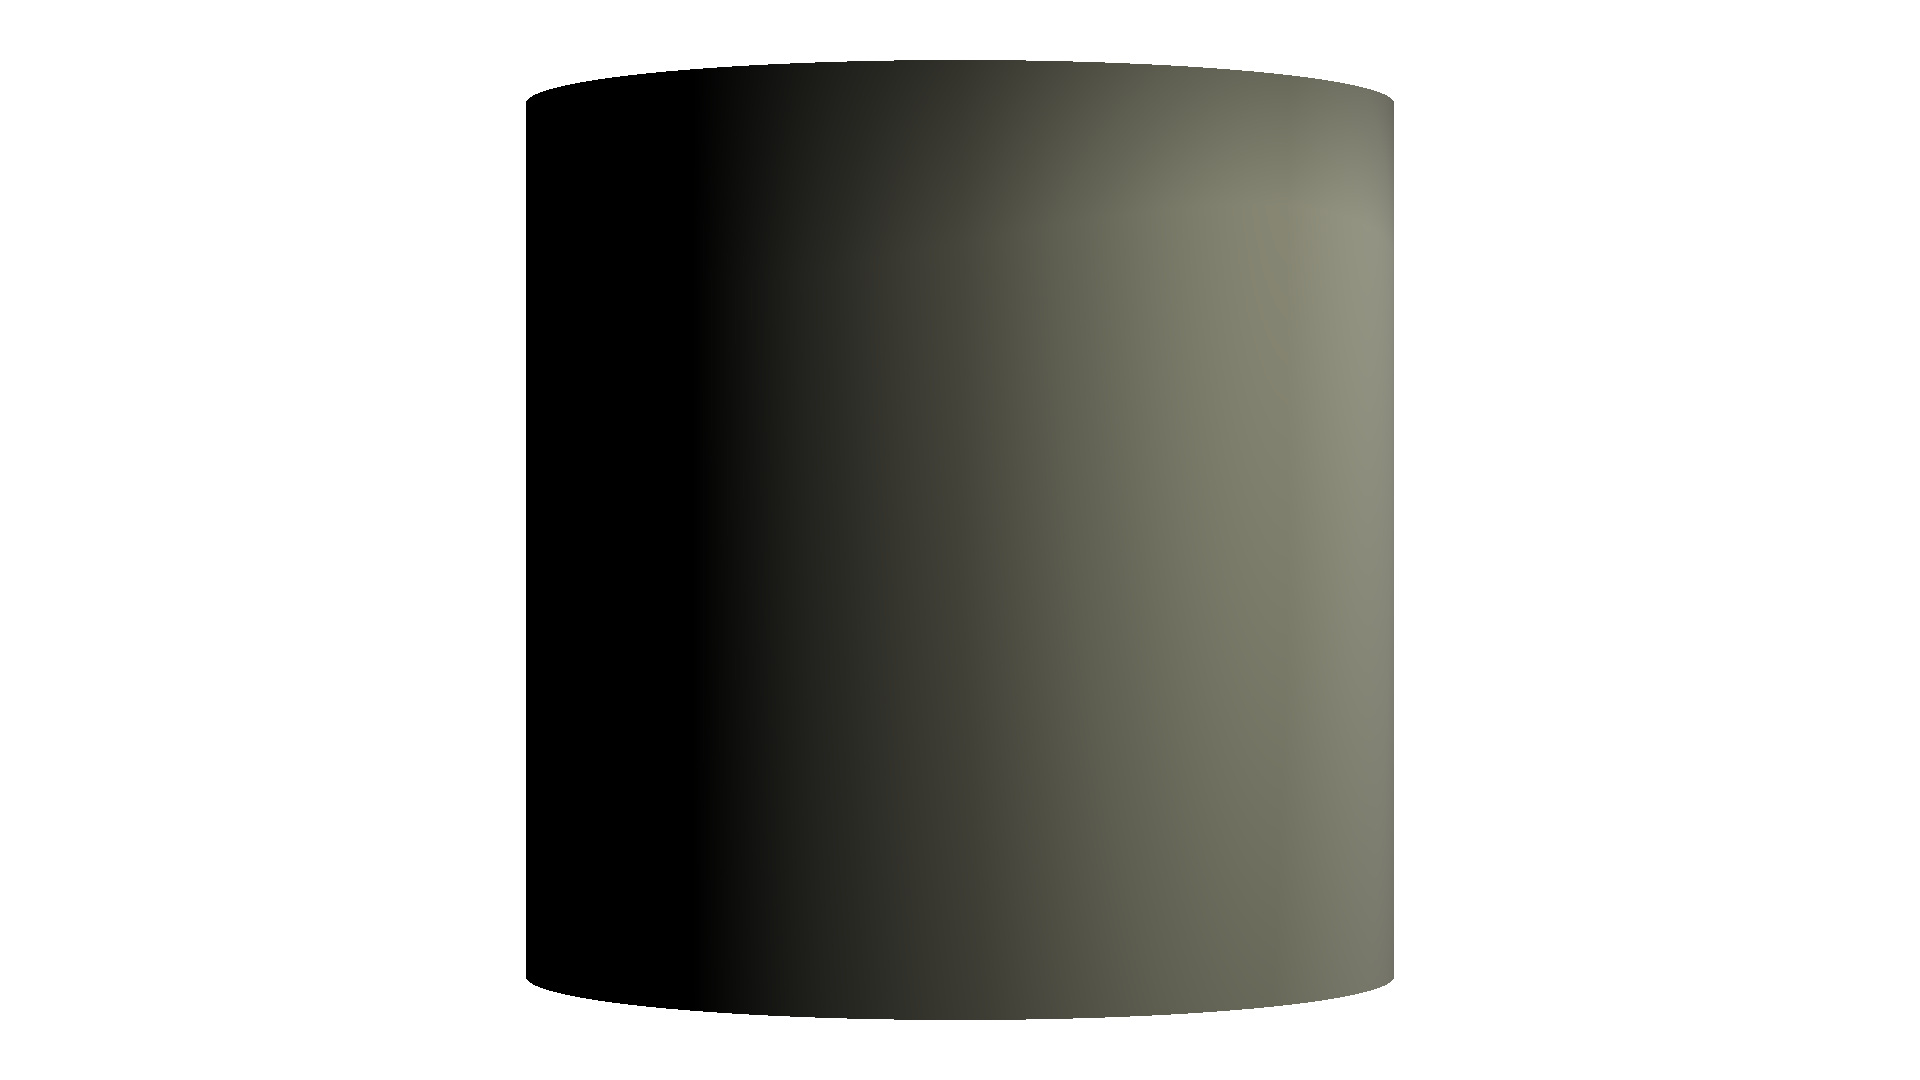
\includegraphics[width=0.45\textwidth]{chapters/ch3/img/BlinnPhong/BP0.png}}
\subfigure{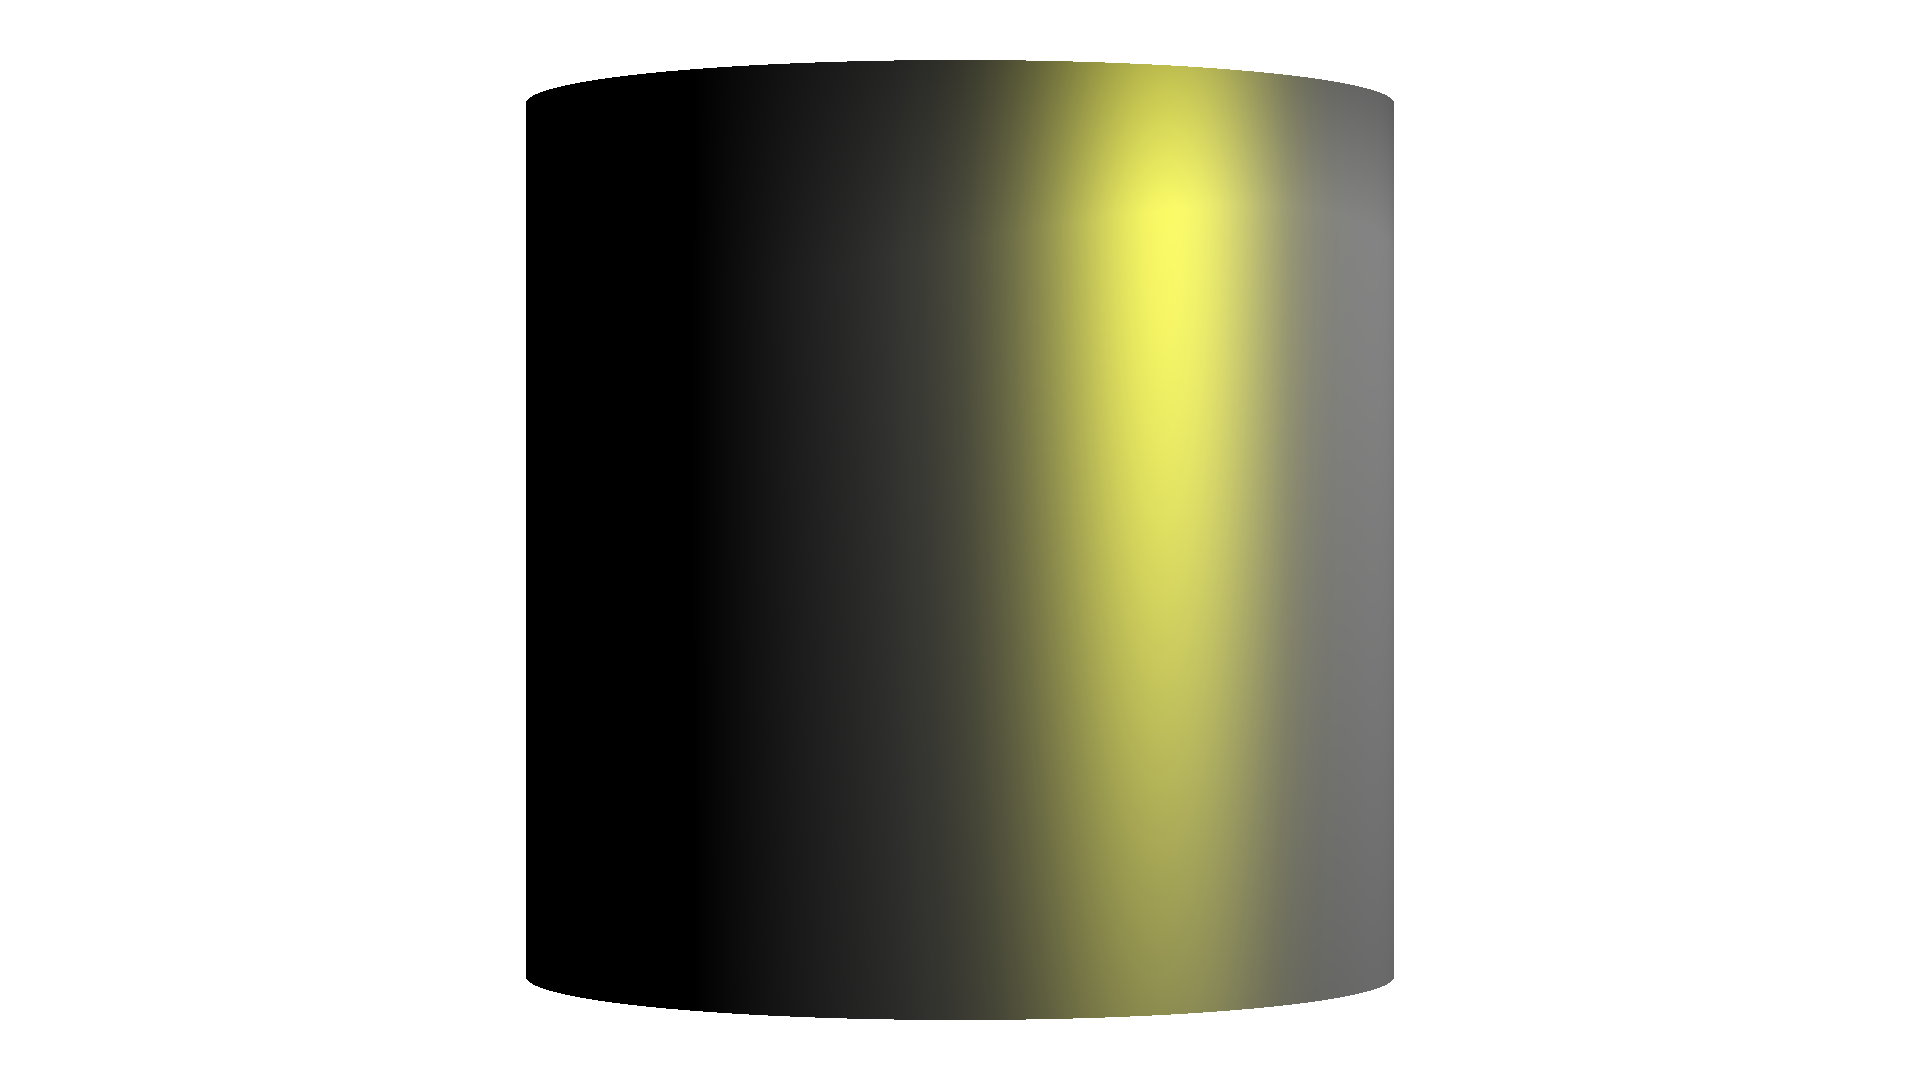
\includegraphics[width=0.45\textwidth]{chapters/ch3/img/BlinnPhong/BP16.png}}
\subfigure{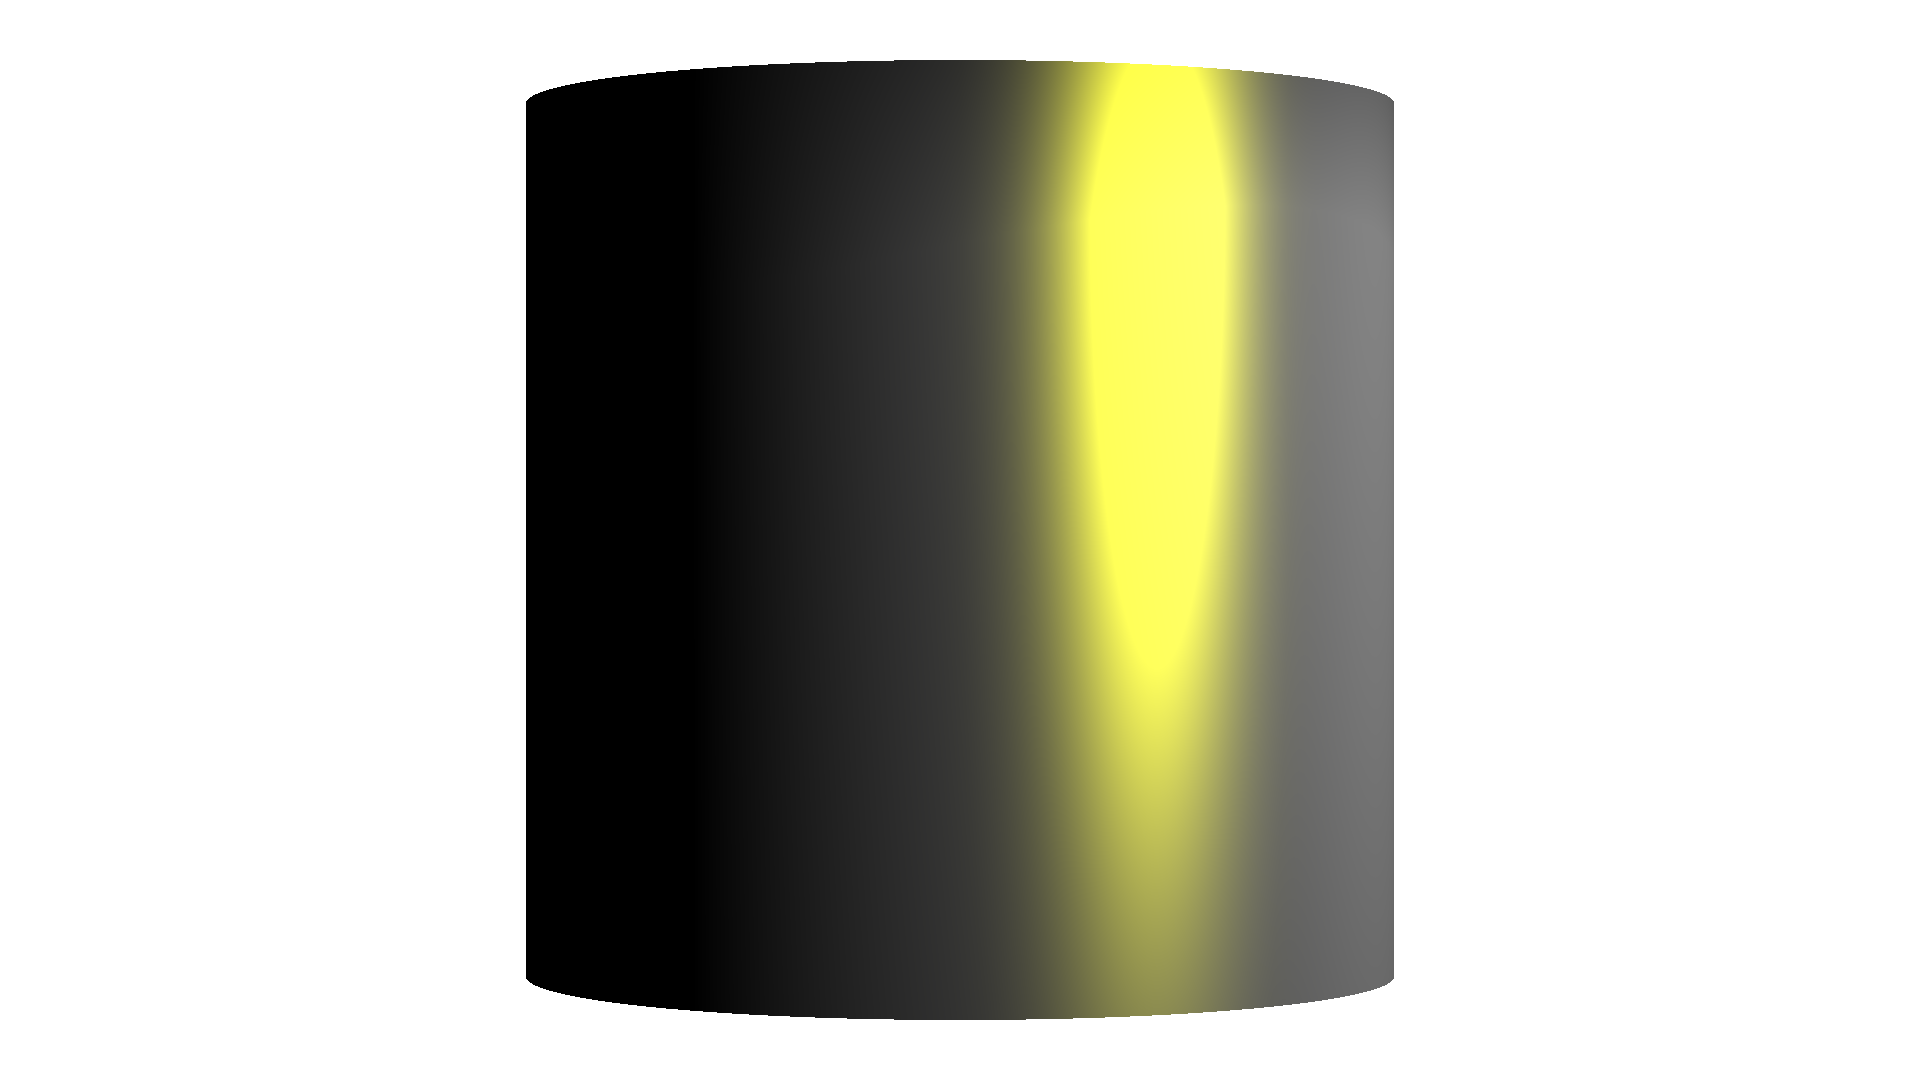
\includegraphics[width=0.45\textwidth]{chapters/ch3/img/BlinnPhong/BP32.png}}
\subfigure{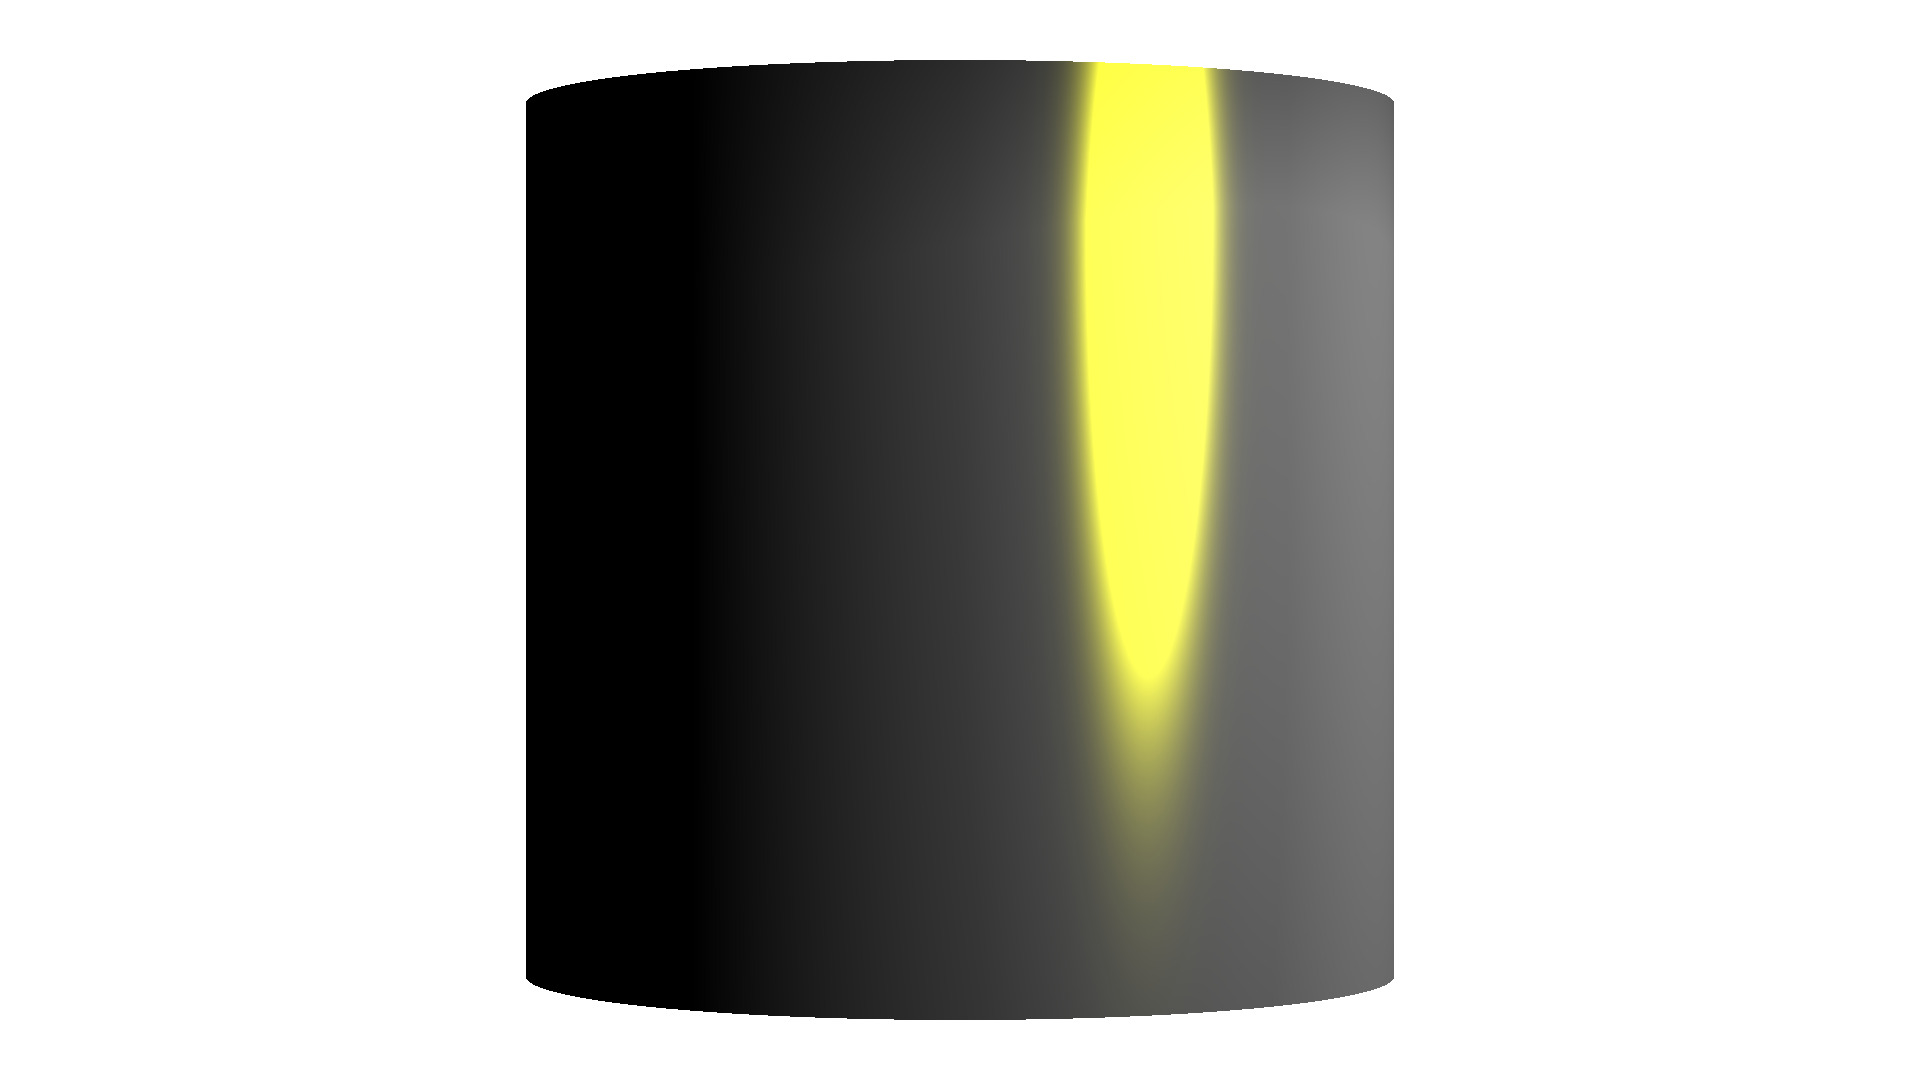
\includegraphics[width=0.45\textwidth]{chapters/ch3/img/BlinnPhong/BP128.png}}

\caption[Rola parametru rozbłysku $e$ w modelu Blinna-Phonga]{Rola parametru rozbłysku $e$ w modelu Blinna-Phonga. Idąc od lewej do prawej z góry na dół parametr $e$ przyjmuje następujące wartości: 0, 16, 32, 128. Z uwagi na fakt, iż~kolory zapisywane są w postaci 24-bitowych wartości, gdzie każda z trzech składowych \texttt{RGB} reprezentowana jest przez 8 bitów, na obrazach dostrzec można efekty związane z obcięciem wartości do 255, które objawiają się jako obszary rozbłysku o jednakowym kolorze.}
\label{ch3:img:blinn_phong}
\end{figure}